% Chaptre 1

\chapter{Approche suivie et solution proposée} % Main chapter title

\label{Chaptre4} % For referencing the chapter elsewhere, use \ref{Chapter1} 

Dans cette section nous ferons une présentation détaillée des solutions que nous avions proposées par rapport à nos missions.

%----------------------------------------------------------------------------------------

% Define some commands to keep the formatting separated from the content 
%\newcommand{\keyword}[1]{\textbf{#1}}
%\newcommand{\tabhead}[1]{\textbf{#1}}
%\newcommand{\code}[1]{\texttt{#1}}
%\newcommand{\file}[1]{\texttt{\bfseries#1}}
%\newcommand{\option}[1]{\texttt{\itshape#1}}
%----------------------------------------------------------------------------------------

\section{Méthodologie de travail: Scrum avec Agile}
L’agrandissement de l’équipe tech et le besoin de fournir des livrables réguliers pour montrer l’évolution aux fonds d’investissement a nécessité la mise en place d’une nouvelle méthodologie de travail avec la méthode Agile Scrum.\\ \\ La méthode Agile est organisée en cycles de développements itératifs qui place le produit avant le projet. L’objectif n’est pas de terminer le projet mais de mettre en place un produit fini qui répond à toutes les exigences du client. Cette méthode part du principe que les besoins ne sont pas figés et peuvent évoluer avec le projet.\\ \\L’objectif final n’est pas défini au départ du projet mais des objectifs sont définis à court terme et fonctionne par étape. Une fois atteinte, un point est fait, les améliorations possibles sont mises en avant et l’étape suivante est définie en conséquence. Ce processus est ensuite répété jusqu’à l’obtention du produit final répondant à toutes les attentes. Avec ce fonctionnement, le client devient acteur du projet et peut être sollicité à chaque étape. Chaque étape doit durer 2-3 semaines maximum, comprenant des phases de test et le produit en sortie est incomplet mais doit être fonctionnel.\\ \\ La méthodologie Scrum reprend le cadre de travail Agile pour des projets plus complexes. Le projet est décomposé en «sprints» qui sont les étapes de développement. Afin de produire des livrables régulièrement et rapidement, nos sprints duraient une semaine.Une réunion est mise en place à chaque début de sprint afin de définir les objectifs de la semaine et leurs priorités. Durant toute la durée du sprint, une réunion quotidienne d’une durée de 30 minutes, « standup », a lieu, dans l’idée les participants restent debout pour éviter de s’éterniser. Chaque participant prend la parole afin de présenter son travail de la veille, valider les objectifs terminés et définir ceux du jour. Cette courte réunion doit servir à mettre en avant les points de blocage et synchroniser tous les membres de l’équipe. Le Scrum Master, chargé de vérifier le bon déroulement du sprint, doit valider avec l’équipe si les délais peuvent toujours être tenus et si le sprint est toujours réalisable dans son intégralité.\\ \\
Chaque fin de sprint comprend un point sur tous les objectifs validés ainsi qu’une démonstration du travail réalisé durant la semaine. Dans notre cas, un test de l’application est effectué afin d’obtenir des retours de tous les membres de l’équipe tech. Ces remarques seront ensuite prises en compte ou non dans le prochain sprint.
\subsection{Les principaux rôles de la méthodologie Scrum}
\begin{list}{•}
\item  \textbf{ Product Owner:} il est chargé de la vision du produit à réaliser et de définir les objectifs prioritaires.
\item
\item  \textbf{ Scrum Master:}membre de l’équipe chargé de vérifier la bonne application de la méthodologie de travail, il anime généralement les réunions quotidiennes. Ce rôle n’est pas figé et peut passer d’un membre à l’autre au sein de l’équipe.
\item  \textbf{ L’équipe de développement :}équipe chargée de réaliser les objectifs définis dans le sprint et se composant généralement de profil différent
\end{list}  
\newpage
\section{Les différentes missions et solutions}
\subsection{Mission 1:Etude de faisabilité sur le déploiement d’une application Front-End dans un environnement AWS}
L’application frontend(web app flutter) de Gighamesh est hébergée sur Firebase, tandis que l’essentiel de
ses ressources se trouve dans le cloud d’Amazon. C’est dans le but d’unifier nos environnements cloud que
cette mission m’avait été confiée.
\subsubsection{Observations}
Les applications web Flutter sont  développées avec le langage de programmation Dart. Avant le déploiement d'une application Flutter un build est nécessaire, 
et le résultat de celui-ci est un ensembles des fichiers statiques( html, css, js, ...). Ce sont ces fichiers statiques qui sont déployés.
Pour résoudre  j’avais exploré deux possibilités:
\subsubsection{Solutions}
\subparagraph{Solution1: L’utilisation de S3 comme repos de d'hébergement}
La solution ici consiste à créer un repos S3, de le rendre public, afin de pouvoir accepter tous les trafics.
De configurer Code Pipeline pour les besoins de CI/CD avec Github, De configurer Cloudfront pour la
gestion du trafic et Route 54 pour le routage.
 \begin{figure}[H]
            \centering
                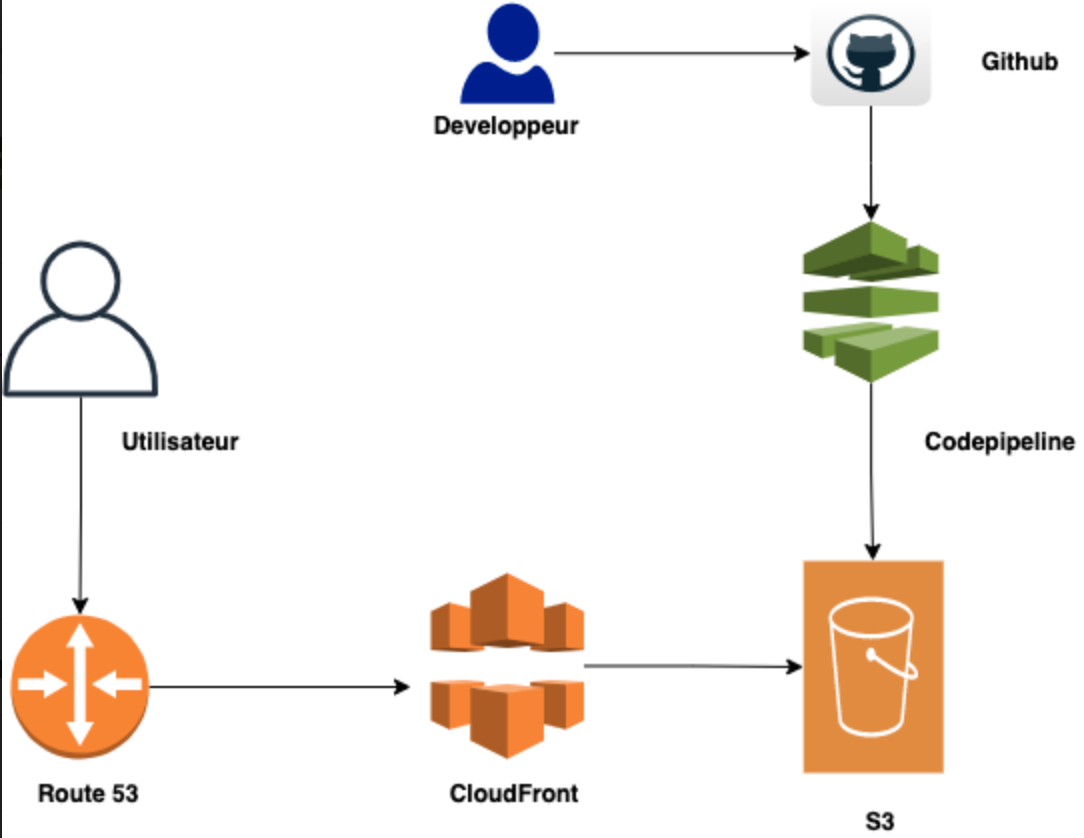
\includegraphics[width=0.8\textwidth]{Figures/S3}
	       \decoRule
		\caption[Solution à base de S3]{Solution à base de S3}
	\label{fig:S3}
	\end{figure}
\newpage
\subparagraph{Solution2: L’utilisation d’Amplify comme comme repos d'hébergement}
Cette solution consiste à utiliser le service d’hébergement qu’offre Amplify et son système de CI/CD en
l’associant au système de versioning: Github. J'avais utilisé CloudFront pour la gestion du trafic et Route 54
pour le routage.
NB: C’est la solution 2 qui avait été retenue. Celle-ci est simple et plus adaptée.
 \begin{figure}[H]
            \centering
                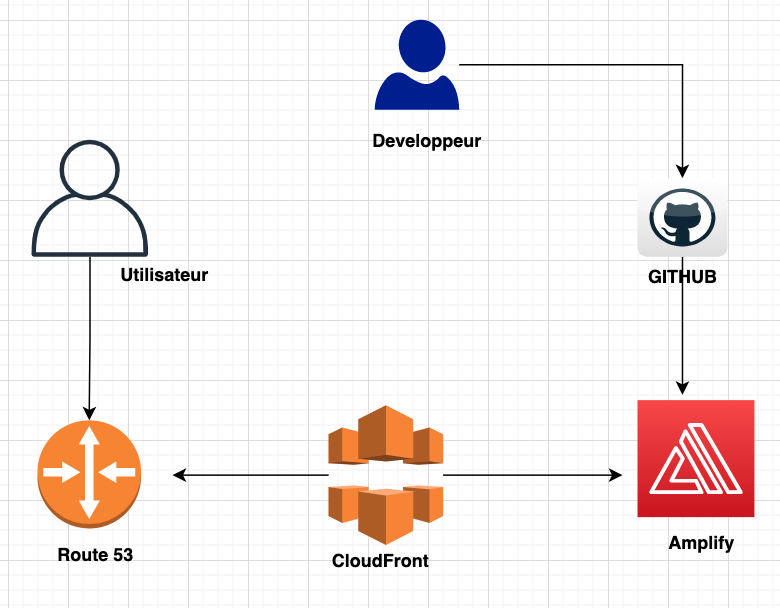
\includegraphics[width=0.8\textwidth]{Figures/amplify}
	       \decoRule
		\caption[Solution à base d'Amplify]{Solution à base d'Amplify}
	\label{fig:Amplify}
	\end{figure}
	
\subsection{Mission 2:Le déploiement et l’intégration du service web (Reflex) dans le parcours de souscription}
La souscription au produit d’assurance Assurly est subdivisée en trois parcours: P1, P2, et P3. Un utilisateur ne peut se
retrouver que dans un seul parcours en fonction des données fournies. Si un utilisateur se retrouve dans le
parcours P3 un questionnaire plus complexe est nécessaire, c’est à cet instant qu’intervient Reflex.
\newpage
\subsubsection{Solutions}
%Reflex est composé de trois modules de base: CEP pour frontend, DOCS pour la gestion des rapports et
%RAS qui constitue le cœur du système Reflex.
%La procédure de déploiement consiste mettre à jour le repos Github qui contient les fichiers nécessaires à la
%construction de notre container, à se connecter à notre EC2, à puller les fichiers du repos Github depuis un
%répertoire de notre EC2 puis à construire et déployer notre container avec la commande docker-compose.
\subsubsection{Pipeline de déploiement}
Quand nous recevons de notre partenaire des mises à jour des modules Reflex , nous les déployons(push) sur un repos Github. Notre repos Github est connecté à notre docker hub; ce qui déclenche automatiquement la construction et le déploiement(push) de l'image de notre conteneur sur docker hub. Pour déployer Reflex sur notre EC2: Il suffit soit de récupérer(pull) le contenu du repos Github puis construire l'image et déployer le conteneur ou de récupérer(pull) l'image de docker hub puis déployer le conteneur. La figure ci-dessous illustre le processus.  
 \begin{figure}[H]
            \centering
                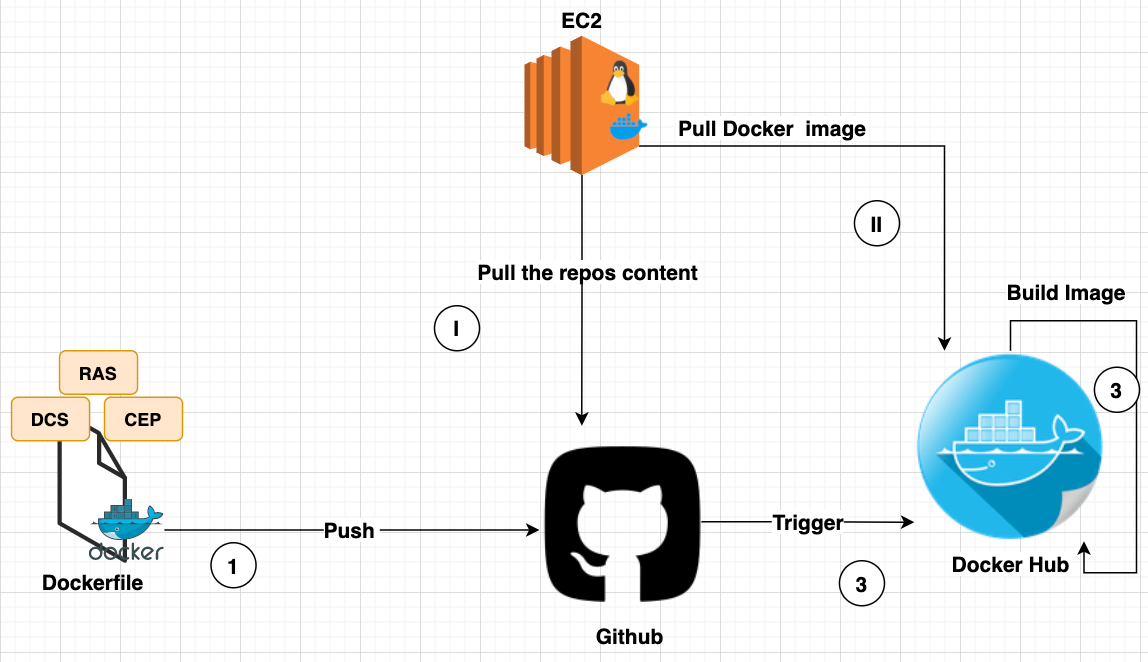
\includegraphics[width=0.8\textwidth]{Figures/pipeline1}
	       \decoRule
		\caption[Pipeline de déploiement de Reflex]{Pipeline de déploiement de Reflex}
	\label{fig:Pipeline de déploiement de Reflex}
\end{figure}

 \begin{figure}[H]
            \centering
                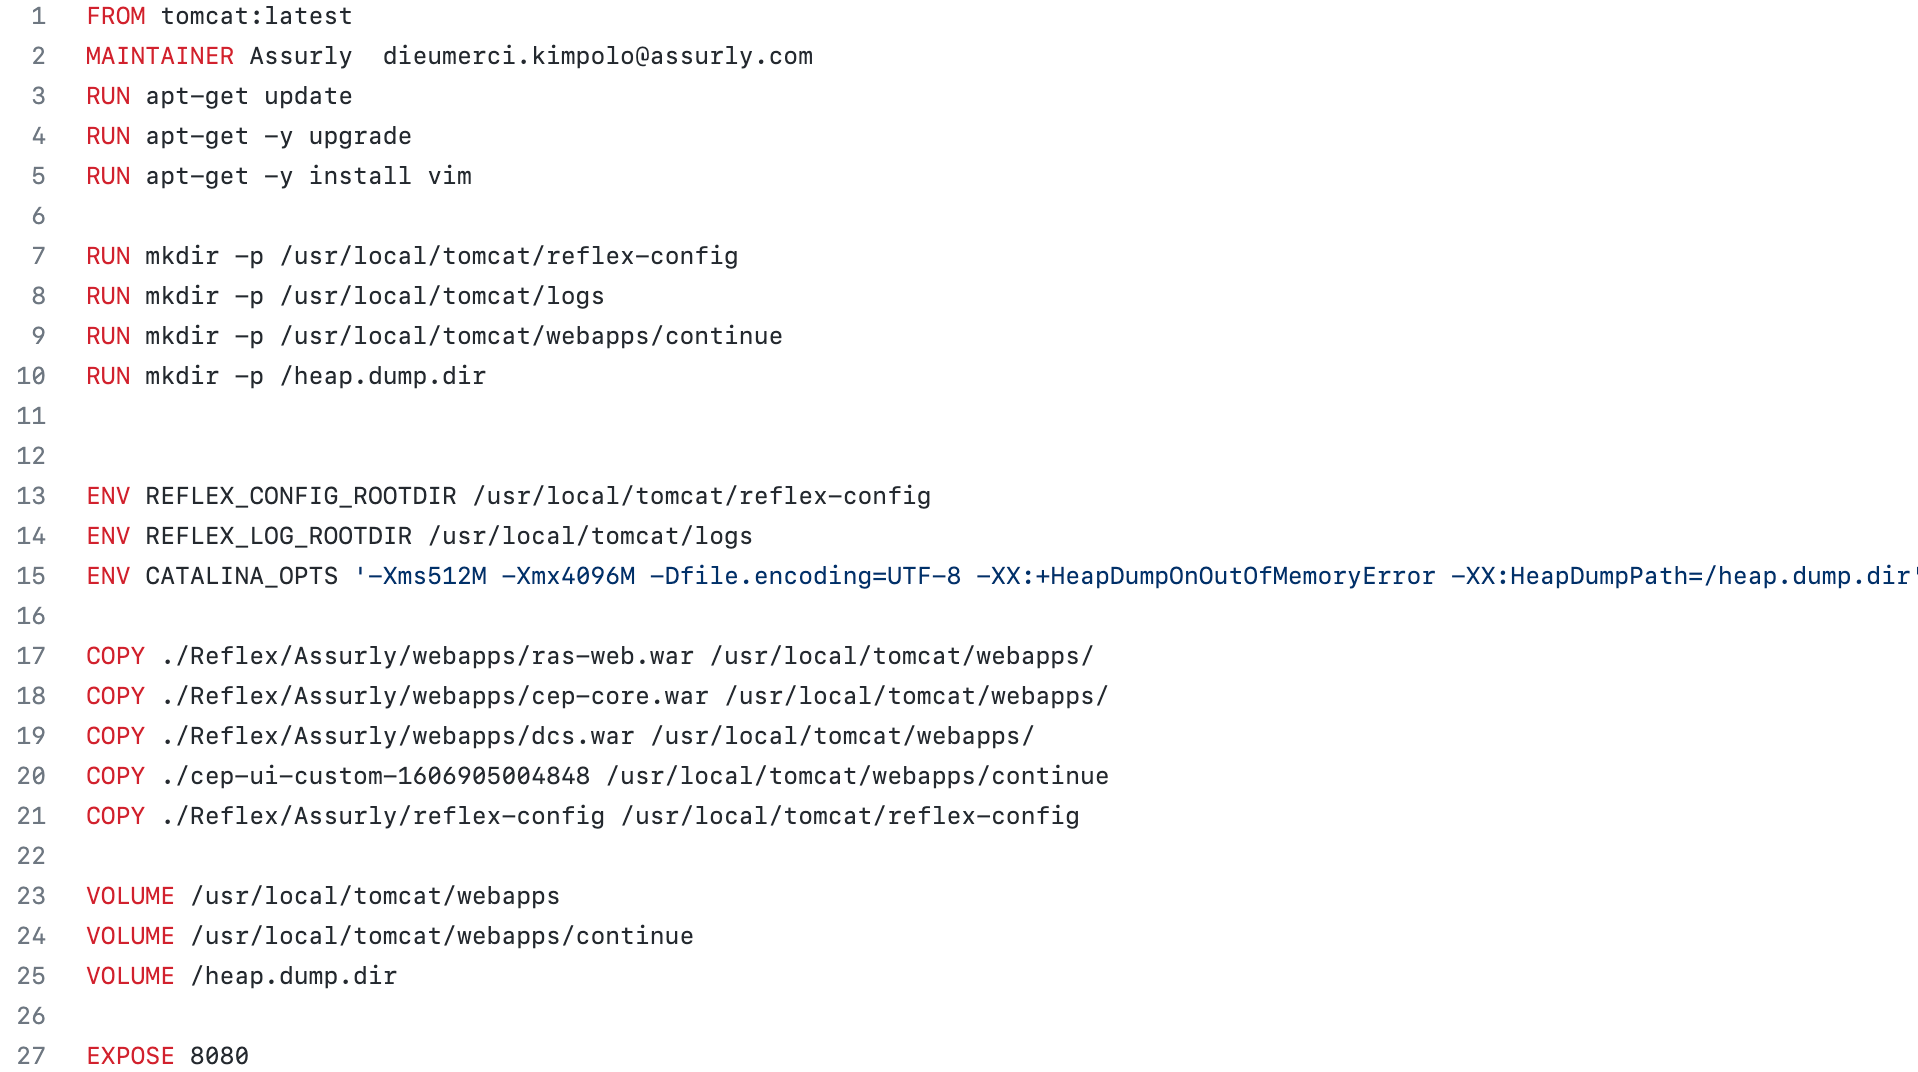
\includegraphics[width=0.8\textwidth]{Figures/dockerfile}
	       \decoRule
		\caption[Dockerfile de construction de l'image Reflex]{Dockerfile de construction de l'image Reflex}
	\label{fig:Dockerfile de construction de l'image Reflex}
\end{figure}
\newpage
\subsubsection{Diagramme de séquence intégration}
L'intégration de Reflex sur l'application web est différente de celle sur l'application mobile.

\textbf{Cas de l'application web}
Notre application web est embarquée dans une Iframe, et l'intégration de Reflex passe par une initialisation des cookies. Il nous était impossible d'initialiser les cookies d'un autre domaine depuis l'Iframe de notre application web. Pour palier ce problème nous avons développé une application intermédiaire hébergée sur le même server web que le moteur Reflex. Les utilisateurs en P3 qui passe par notre application web sont redirigés  sur  l'application web intermédiaire, pour soumettre leur questionnaire Reflex et sont redirigés sur l'application web depart à la fin du processus. Le BACKEND sur le diagramme de séquences ci-dessous représente notre infrastructure dans l'environnement AWS.
 \begin{figure}[H]
            \centering
                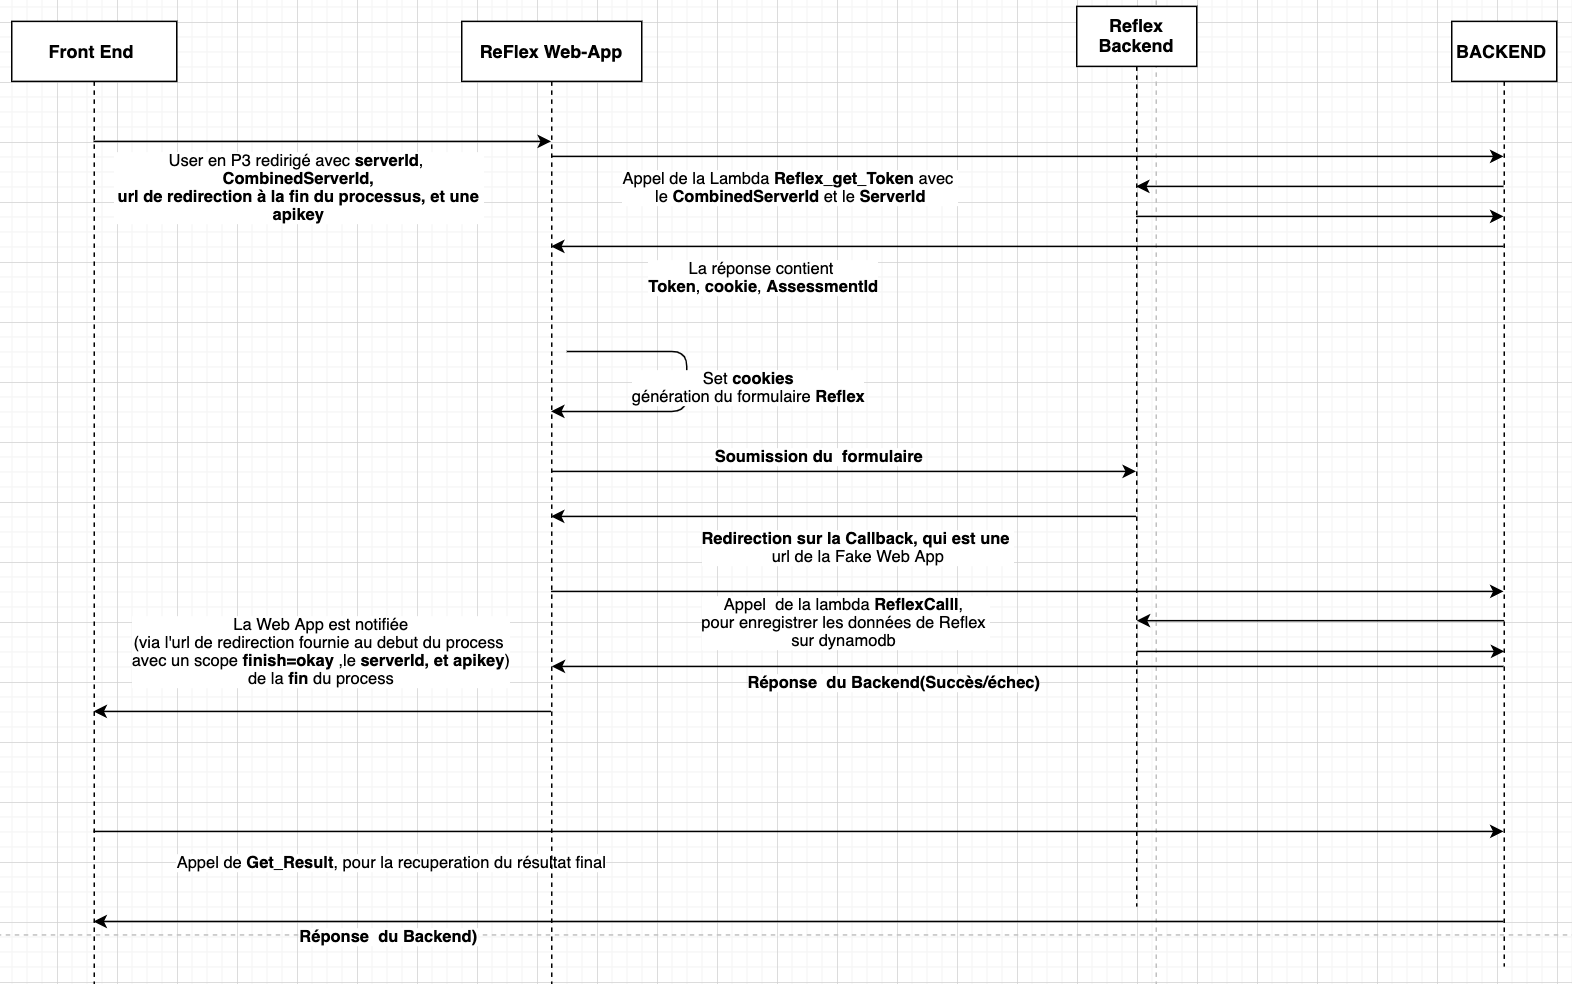
\includegraphics[width=0.8\textwidth]{Figures/reflexweb}
	       \decoRule
		\caption[Diagramme d'intégration de Reflex sur l'application web]{Diagramme d'intégration de Reflex sur l'application web}
	\label{fig:Diagramme d'intégration de Reflex sur l'application web}
\end{figure}

 \begin{figure}[H]
            \centering
                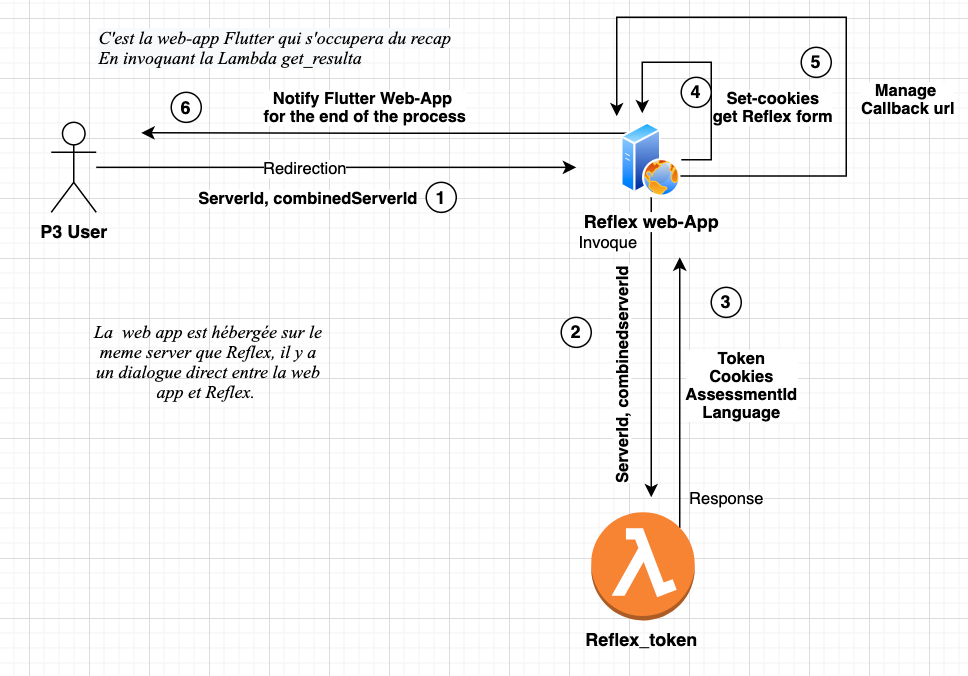
\includegraphics[width=0.6\textwidth]{Figures/reflexapp}
	       \decoRule
		\caption[Diagramme d'intégration de Reflex sur l'application web]{Diagramme d'intégration de Reflex sur l'application web}
	\label{fig:Diagramme d'intégration de Reflex sur l'application web}
\end{figure}
\newpage
\subsection{Mission 3: Etude de la sécurité actuelle d’accès aux API}
Les API sont devenues incontournables, il existe très peu ou presque pas de systèmes informatiques qui ne consomment et/ou ne fournissent des API. Dans la plus part des cas ou très souvent on est soit consommateur, soit fournisseur  ou les deux.\\ \\ Comme les applications classiques, les API n'échappent pas au problèmes de sécurité. Elles font face aux mêmes défis que les applications ordinaires. Elles sont vulnérables à plusieurs types  d'attaques comme: les attaques Dos et attaques par pollutions des paramètres http,...\\ La question de sécurité des API comme pour des applications ordinaires doit être pris en considération durant tout le cycle son développement: de sa conception à sa mise en production. \\Dans le cadre de mon étude je m'était focalisé sur les API de type Rest conçues et et déployées dans le cloud d'Amazon.\\ Dans l'environnement AWS les Backend des API sont protégés par le service API Gateway, et une très grande parties des protocoles de sécurité y sont implémentés.
\subsubsection{Rappel des principes de sécurité}
Un système sécurisé doit garantir les points suivants:
\begin{itemize}
\item \textbf{L'intégrité:} garantir que les données sont bien celles que l'on croit être
\item \textbf{La disponibilité:} maintenir le bon fonctionnement du système d'information
\item \textbf{La confidentialité:} rendre l'information inintelligible à d'autres personnes que les seuls acteurs d'une transaction
\end{itemize}
\subsubsection{La sécurité des API dans AWS}
Pour sécuriser une API dans l'environnement AWS il faut prendre en compte deux aspects suivants: 
\begin{enumerate}
\item Les contrôles d'accès 
\item L'authentification et les autorisations
\end{enumerate}
Il n'ya pas de choix à faire entre les contrôles d'accès et le système d'authentification \& d'autorisation, ils sont complémentaires.
\subsubsection{Les contrôles d'accès}
Les mécanismes suivants peuvent être utilisés pour effectuer d'autres tâches liées au contrôle de l'accès aux API dans AWS.
\begin{list}{•}
\item \textbf{Le partage des ressources cross-origin (CORS)}  permet de contrôler la façon dont votre API REST répond aux requêtes de ressources inter-domaines. 
\item
\item \textbf{Les certificats SSL côté client} peuvent être utilisés pour vérifier que les requêtes HTTP adressées à votre système backend proviennent d'API Gateway.
\item \textbf{AWS WAF} peut être utilisé pour protéger votre API d'API Gateway contre les menaces web courantes telles que l'injection SQL et les attaques XSS (cross-site 
scripting). 
\item \textbf{API Key} peut être utilisé pour gérer les quotas des appels de l'API
\item \textbf{API endpoints  ressorces policy} peut être utilisé pour refuser certains appels en fonction des adresse IP
\item \textbf{VPC endpoints policy } peut être utilisé pour gérer les endpoints accessibles seulement pour les adresse IP privées
\end{list}
 \begin{figure}[H]
            \centering
                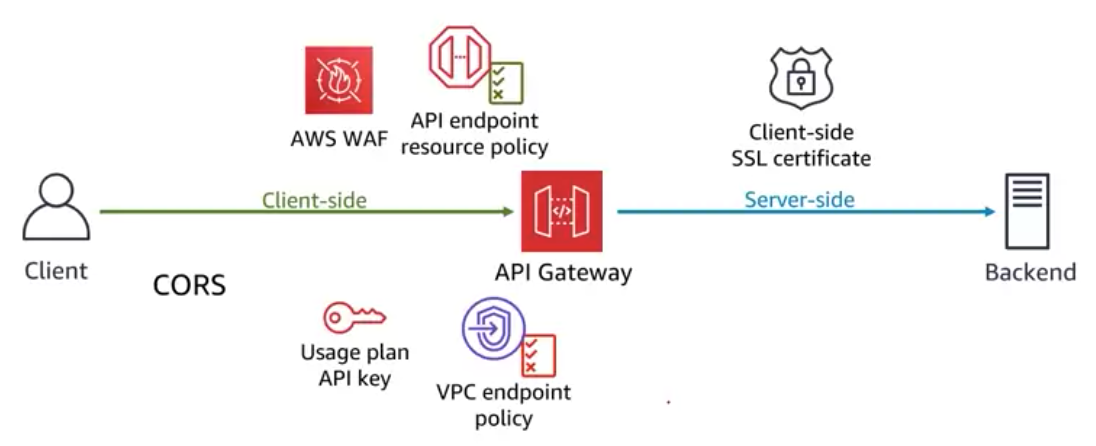
\includegraphics[width=0.8\textwidth]{Figures/controleaccess}
	       \decoRule
		\caption[Les contrôles d'accès]{Les contrôles d'accès}
	\label{fig:Les contrôles d'accès}
	\end{figure}
%\textbf{Password grant}
\subsubsection{Authentification et autorisations}
Le protocole de base de gestion des authentifications et des autorisations au niveau des API Rest est le protocole Oauth2, décrit dans la section état de l'art. Aws utilise essentiellement le service Cognito pour gérer les questions d'autorisation et d'authentification sur des API. Cognito dans son fonctionnement suit les principes de base du protocole Oauth2. 
%C'est Cognito que nous avons utilisé pour gérer les authentifications et les autorisations. 

\subsubsection{L'existent}

\textbf{Points positifs}\\
L'Api est accessible en https, les CORS et les contrôles d'accès par API Key sont implémentés sur l'API Gateway.
%\begin{enumerate}
%\item L'Api est accessible et https
%\item Implémentation des CORS et la gestion des API key sur l'API Gateway
%\end{enumerate}

\textbf{Points négatifs}\\
Le service Cognito est implémenté  mais consommé via de fonctions Lambda personnalisées, le service Cognito implémenté  et consommé via de fonctions Lambda personnalisées,
les données des utilisateurs filtrées avec des paramètres autres le token d'accès valide aussi un chiffrement  est implémenté sur les applications frontend en plus du ssl. 
%\begin{enumerate}
%\item Le service Cognito implémenté  et consommé via de fonctions Lambda personnalisées
%\item Les données des utilisateurs filtrées avec des paramètres autres le token d'accès valide
%\item Implémentation d'un chiffrement  supplémentaire en dehors du ssl
%\end{enumerate}

\subsubsection{Observations}
\begin{enumerate}
\item Cognito à la base ne peut supporter qu'un seul user pool (support de stockage des utilisateurs) sur une API
\item L'API  est  type Rest et déployé dans le cloud d'Amazon
\item Les utilisateurs  stockés dans  plusieurs users pool
\item L'API est consommée par des applications web et  mobiles
\end{enumerate}
Pour supporter plusieurs user pools sur nos API, nous avons développé un système d'autorisation personnalisé à base d'une Lambda. Dans notre implémentation nous avons exploré deux flows: l'implicit grant(en utilisant la web UI de Cognito) et password grant.

%L'intégrité : garantir que les données sont bien celles que l'on croit être. La disponibilité : maintenir le bon fonctionnement du système d'information. La confidentialité : rendre l'information inintelligible à d'autres personnes que les seuls acteurs d'une transaction.
\textbf{Implicit grant}
 \begin{figure}[H]
            \centering
                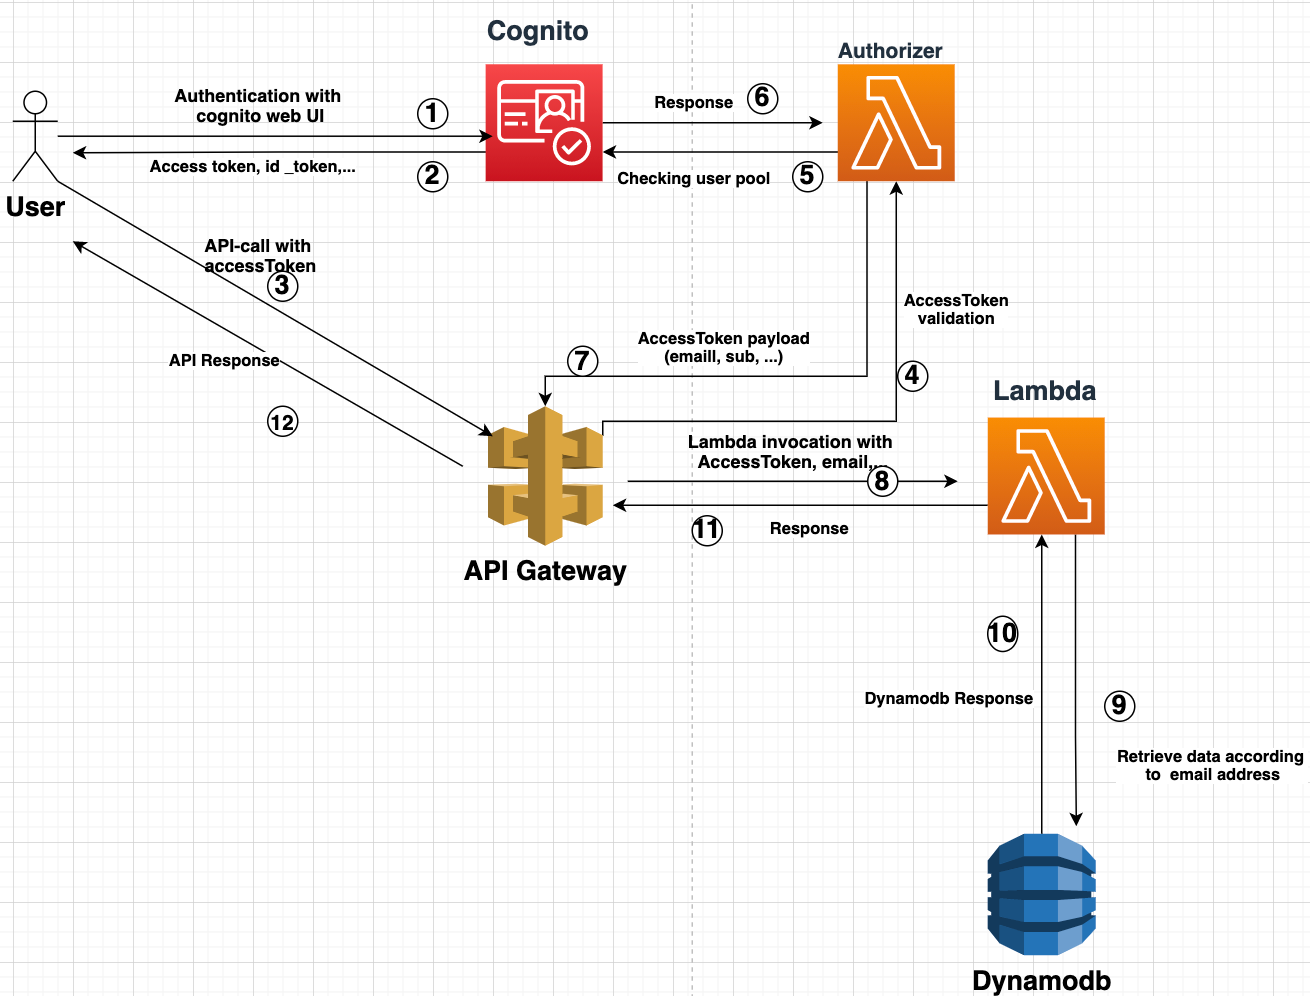
\includegraphics[width=0.8\textwidth]{Figures/securite}
	       \decoRule
		\caption[L'architecture du système de sécurité, Implicit grant]{L'architecture du système de sécurité, Implicit grant}
	\label{fig:L'architecture du système de sécurité, Implicit grant}
	\end{figure}
%\textbf{Password grant}
 
\newpage
\subsection{Mission 4(Mise en place d'un ETL d'intégration de données)}
Gigamesh disposait une quantité importantes des données stockées dans des fichiers txt; des données nécessaires pour effectuer des campagnes de marketing ciblées. Ma mission consistait à intégrer ces données dans une base de données sql pour pouvoir y effectuer facilement  des requêtes.

\subsubsection{Observations}
\begin{enumerate}
\item Tous les fichiers avaient la même structure
\item Le caractère | était utilisé comme séparateur des colonnes
\item Les libellés des colonnes étaient de fois des phrases
\item Les données n'étaient pas typées
\end{enumerate}
\subsubsection{Solution}
Pour résoudre le problème j'avais mise en place un \textbf{ETL}, qui récupère les données brutes(fichiers txt) de leur support de stockage, les transforme avec un \textbf{script Python} et les stocke dans base de données Mysql dans l'environnement AWS via le service Aurora. 

 \begin{figure}[H]
            \centering
                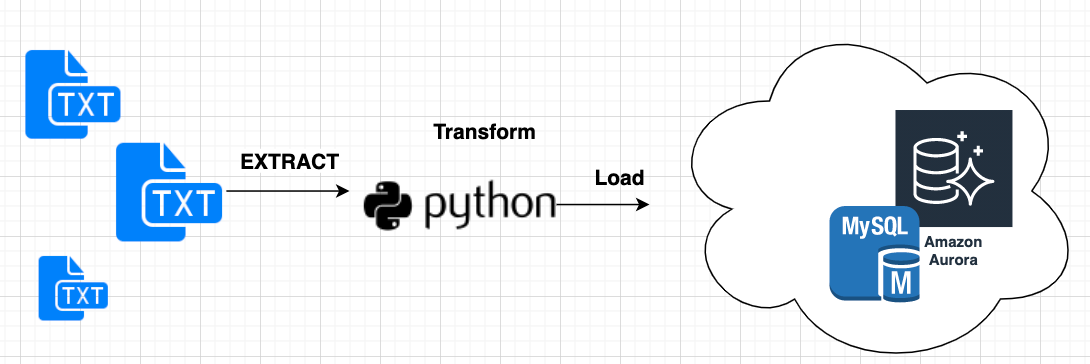
\includegraphics[width=0.8\textwidth]{Figures/etls}
	       \decoRule
		\caption[Etl d'intégration de données]{Etl d'intégration de données}
	\label{fig:etl}
	\end{figure}
La partie de transformation de mon ETL m'avait servi à la création de la table où sont stockées les données et à leur typage. 
 \begin{figure}[H]
            \centering
                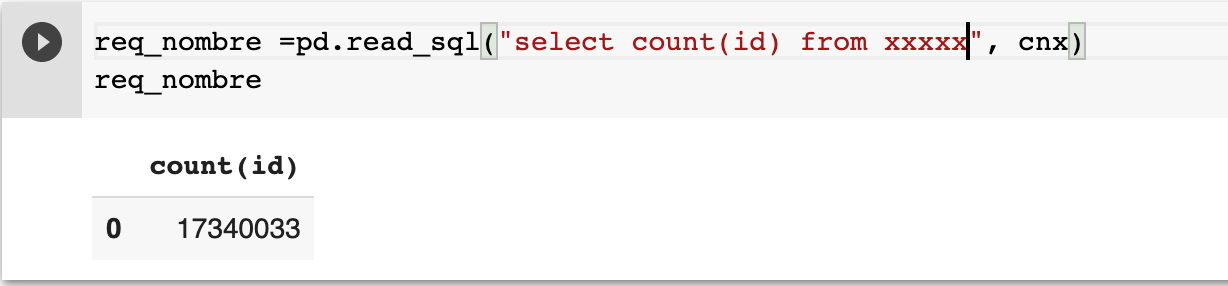
\includegraphics[width=0.8\textwidth]{Figures/nombre}
	       \decoRule
		\caption[La taille de la table où sont stockées nos données]{La taille de la table où sont stockées nos données}
	\label{fig:La taille de la table où sont stockées nos données}
	\end{figure}
